\documentclass[crop,tikz]{standalone}
\usepackage{tikz}

\usetikzlibrary{positioning}

\begin{document}
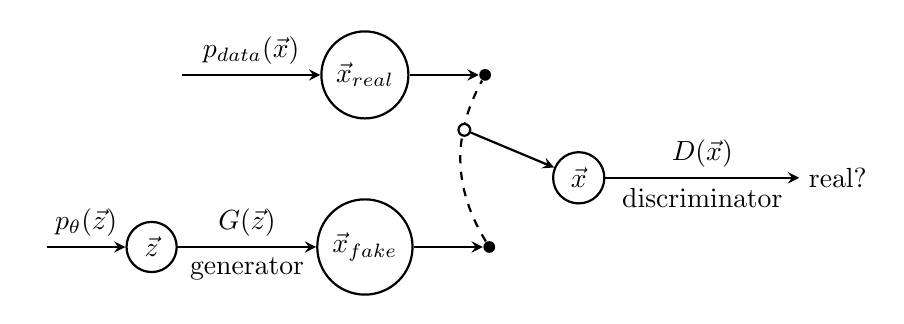
\begin{tikzpicture}

	\node[circle, draw, thick] (z) {$\vec{z}$};
	\node[circle, draw, thick, right=5em of z] (x) {$\vec{x}_{fake}$};
	\draw[-stealth, thick] (z) -- node[above] {$G(\vec{z})$} node[below] {generator} (x);
	\node[left=of z] (i) {};
	\draw[-stealth, thick] (i) -- node[above] {$p_\theta(\vec{z})$} (z);
	\node[above=of x, circle, draw, thick] (xt) {$\vec{x}_{real}$};
	\node[left=5em of xt] (it) {};
	\draw[-stealth, thick] (it) -- node[above] {$p_{data}(\vec{x})$} (xt);
	\node[circle, draw, thick, right=5em of x, yshift=2.5em] (D) {$\vec{x}$};
	\node[right=7em of D] (out) {real?};
	\draw[-stealth, thick] (D) -- node[above] {$D(\vec{x})$} node[below] {discriminator} (out);
			
	\node[right=2.5em of x, circle, fill, inner sep=0.15em] (pt1) {};
	\node[right=2.5em of xt, circle, fill, inner sep=0.15em] (pt2) {};
			
	\draw[dashed, thick] (pt1) edge[bend left] (pt2);
			
	\node[circle, draw, thick, fill=white, inner sep=0.15em] at ([xshift=-0.9em, yshift=4em]pt1.north) (pt3) {};
			
	\draw[-stealth, thick] (x) -- (pt1);
	\draw[-stealth, thick] (xt) -- (pt2);
	\draw[-stealth, thick] (pt3) -- (D);

\end{tikzpicture}
\end{document}